\documentclass[12pt]{article}
\usepackage[letterpaper,margin=1in]{geometry}
\usepackage{hyperref}
\usepackage{amsmath,amssymb}
\usepackage{graphicx}
\begin{document}
\begin{center}
{\bf \LARGE AST1420 ``Galactic Structure and Dynamics'' Final}\\[7pt]
\emph{Due on Apr. 23 by 5pm}\\[7pt]
\end{center}

The full mark for the final includes the oral defense of the problems and questions
listed here. The breakdown is: 80\% written solutions and 20\,\% oral
defense of solutions. The points given for the different problems
below only relate to the 80\,\% written-solutions part of the full
mark.\\

Some of the exercises in this problem set must be solved on a computer
and a good way to hand in the problem set is as a \texttt{jupyter
  notebook}. \emph{Please re-run the entire notebook (with \texttt{Cell
    > Run All}) after re-starting the notebook kernel before sending
  it in}; this will make sure that the input and output are fully
consistent. You can also send in a traditional write-up in LaTeX as a PDF, 
but then you also need to send in well-commented code for how you solved 
the numerical problems. Thus, notebooks are preferred :-)\\

\noindent{\bf Problem 1:} (25 points) Evidence for dark matter. In this class, we 
discussed the evidence for dark matter in galaxies and galaxy clusters that historically
led to the acceptance of the dark matter hypothesis. Among these are Zwicky's observations
of Coma cluster galaxies, the Local Group Timing argument, measurements of the rotation curves 
of spiral galaxies in the nearby Universe, and theoretical arguments regarding the 
stability of galactic disks. In about a page to a page-and-a-half, discuss each of these 
pieces of evidence in detail, their relative strengths and weaknesses in supporting the
dark matter hypothesis, and how these measurements have stood up to further observational 
and theoretical developments.\\

\noindent{\bf Problem 2:} (30 points, 6 each) Short questions.\\

\noindent{\bf (a)} IC 2574 is a low-surface-brightness galaxy whose mass budget near the 
center is dominated by dark matter. Its rotation curve has been measured and found to be 
linearly rising, $v_c \propto r$, within about 6 kpc from its center. What type of 
density profile does that imply for the dark matter at the center of IC 2574?\\

\noindent{\bf (b)} A set of galaxies is orbiting in the potential of a galaxy cluster with mass 
$M$. If we were to increase the mass $M$ by a factor of two, while somehow keeping the 
galaxies' distance to the center the same, what would happen to their velocities?\\

\noindent{\bf (c)} Show that the central value of the gravitational potential of an 
arbitrary razor-thin, axisymmetric disk with surface density $\Sigma(R)$ is given by
\begin{equation*}
\Phi(0,0) = -2\pi\,G\,\int_0^\infty\mathrm{d} R \,\Sigma(R)\,.
\end{equation*}

\begin{figure}[htp]
    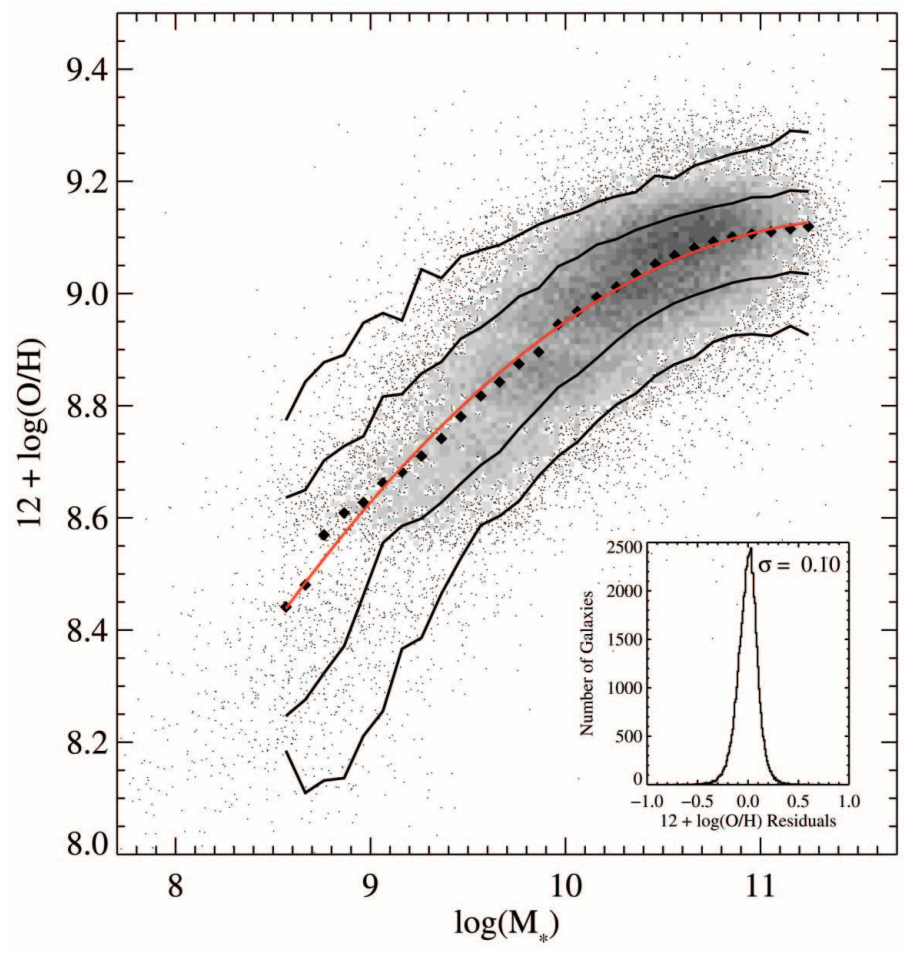
\includegraphics[width=\textwidth]{tremonti.png}
    \caption{The observed mass--metallicity relation for star-forming
      galaxies in the Sloan Digital Sky Survey (Tremonti et
      al. 2004).}\label{fig:tremonti}
    \end{figure}

\noindent{\bf (d)} The observed relation between the oxygen abundance and the stellar 
mass of galaxies is shown in Figure~\ref{fig:tremonti}. It is clear that there is a strong
correlation between the stellar mass and the oxygen abundance for galaxies. Why is 
oxygen a good element to measure to investigate the relation between a galaxy's mass and 
its metal abundance? If you interpret this relation in the context of 
the leaky-box chemical-evolution model, what are two options for
explaining the origin of this relation? Discuss these options in terms
of what we have learned this semester about dynamics and the structure
of galaxies.\\

\noindent{\bf (e)} We derived the dynamical-friction time scale $t_\mathrm{DF}$ in 
Equation (20.74) for an orbit on a circular orbit. For suitably-chosen parameters, 
numerically investigate the effect of eccentricity on $t_\mathrm{DF}$. That is, compare 
$t_\mathrm{DF}$ for objects that spiral in on circular orbits and objects on eccentric 
orbits with the same initial angular momentum. Interpret your results using the 
properties of eccentric orbits and of the dynamical-friction deceleration formula.\\

\noindent{\bf Problem 3:} (25 points; 5 each) A popular method for
modifying gravity is replacing the Newtonian gravitational force with
a \emph{Yukawa force}. In such a model, particles feel a force
mediated through a massive, scalar particle instead of the standard
Newtonian $1/r^2$ force. Such an interaction gives rise to a Yukawa
potential $\Phi_y(r)$; specifically, an object with mass $M$ gives
rise to a potential
\begin{equation}\label{eq:yukawa_pot}
  \Phi_y(r) = -\frac{\alpha\,GM}{r}\,e^{-m_\phi\,r}\,,
\end{equation}
where $\alpha$ parameterizes the strength compared to that of standard
gravity and $m_\phi$ is the mass of the scalar mediator (in the
exponential we are using units in which $\hbar = c = 1$). Let's
investigate these types of models and how well they are constrained!\\

\noindent{\bf{ (a)}} Re-write Equation~\eqref{eq:yukawa_pot} as
\begin{equation}
  \Phi_y(r) = -\frac{\alpha\,GM}{r}\,e^{-r/\lambda}\,,
\end{equation}
by converting $m_\phi$ to a length scale using $\hbar$ and $c$. In
particular, what $m_\phi$ does $10^{12}\,\mathrm{km}$ correspond to
(express $m_\phi$ in eV)?\\

\noindent{\bf{ (b)}} Does Newton's first shell theorem hold if the
gravitational force is of the Yukawa type rather than Newtonian?
Explain why or why not.\\

\noindent{\bf{ (c)}} Explore what orbits look like in a Yukawa
potential. You can do this by considering the effective potential and
looking at orbits that are either near to or far from circular. Some
cases to consider: $r \ll \lambda$, $r = \lambda$, $r = 2\lambda$, and
$r \gg \lambda$.\\

\noindent{\bf{ (d)}} Yukawa-type forces can be constrained by using
the fact that the orbit of the Moon around the Earth or the orbits of
planets around the Sun close to within measurement
uncertainties---after accounting for small deviations stemming from
the general theory of relativity and the Earth/Sun's quadrupole
moment. Compute, analytically, the precession $2\pi-\Delta \psi$ of
the apocenter in a Yukawa potential for a near-circular orbit in terms
of $\alpha$, $\lambda$, and the radius $r$ of the circular orbit. From
observations of Mercury and Mars' orbits, we can determine that
$|2\pi-\Delta \psi| \lesssim 100$ nanoradians. For $\alpha \approx
1$---i.e., gravity is fully Yukawa---what constraint does this put on
$\lambda$ (express in km) and, thus, $m_\phi$ (express in eV)? For
reference, the LIGO constraints on $m_\phi$ are $m_\phi \lesssim
10^{-22}\,\mathrm{eV}$ (these come from the fact that a massive
graviton leads to frequency-dependent travel-times for gravitational
waves, constrained by the observed binary-black-hole mergers, and to a
slower propagation speed of gravitational waves compared to the speed
of light, constrained by the near-coincidence of the
gravitational-wave and electromagnetic emission in the binary
neutron-star merger GW170817).\\

\noindent{\bf{ (e)}} Rather than being a full-on replacement of
Newtonian gravity, Yukawa-type forces may also be present \emph{in
  addition} to gravity. For example, in some dark matter models, dark
matter feels an additional Yukawa force (with strength $\alpha$
relative to Newtonian gravity) in addition to standard gravity, while
ordinary matter does not feel the additional force.  At scales $r \gg
m_\phi^{-1}$, such a force acts as an additional gravitational force
between dark-matter particles and can therefore be modeled as a simple
change in the gravitational constant for such particles: $\tilde{G} =
G\,(1+\alpha)$. Discuss how this additional interaction affects the
following types of observations if we interpret them assuming that
gravity is the only force (that is, how does the inferred mass relate
to the true mass):

\begin{itemize}
\item The matter distribution in disk galaxies inferred from their
  rotation curves.
\item The mass of the Milky Way inferred from the velocities of halo globular clusters.
\item The mass of the Milky Way inferred by assuming that a distant satellite (e.g., Leo I) moves at the escape velocity.
\item The mass of the Local Group determined using the timing
  argument.
\end{itemize}


\end{document}
